% ============================================================
%  OPTIMIZATION STRATEGY
% ============================================================

The LBR design optimization is governed by a two-level strategy. At the conceptual level, the competition between plutonium breeding and burning is framed as a transmutation kinetics problem that establishes the necessary conditions on the neutron spectrum. At the engineering level, those conditions are translated into specific moderator and geometry choices through a sequence of scoping calculations of increasing fidelity, culminating in the full Monte Carlo design iteration described in Section~\ref{sec:neutronics}.

% ============================================================
\subsection{Transmutation Kinetics}
\label{sec:transmutation-kinetics}
% ============================================================

The competition between plutonium production and destruction can be modeled through coupled Bateman equations. Assuming complete decay of $^{239}$Np to $^{239}$Pu ($t_{1/2} = 2.36$\,days, negligible relative to operational timescales), the transmutation dynamics reduce to:

\begin{align}
    \frac{dN_\text{U238}}{dt}  &\approx -\lambda_1 N_\text{U238}(t) \label{eq:U238-ode} \\
    \frac{dN_\text{Pu239}}{dt} &\approx \lambda_2 N_\text{U238}(t) - \lambda_3 N_\text{Pu239}(t) \label{eq:Pu239-ode}
\end{align}

\noindent where the flux-averaged microscopic reaction rates are:
\begin{equation}
    \lambda_1 = \Phi_0 \langle \sigma_\text{a,U238} \rangle, \qquad
    \lambda_2 = \Phi_0 \langle \sigma_{(n,\gamma),\text{U238}} \rangle, \qquad
    \lambda_3 = \Phi_0 \langle \sigma_\text{a,Pu239} \rangle
\end{equation}
with $\Phi_0$ the scalar neutron flux and $\langle \sigma_* \rangle$ denoting flux-averaged microscopic cross sections. Uranium-238 depletion follows exponential decay:
\begin{equation}
    N_\text{U238}(t) = N_\text{U238}(0)\,e^{-\lambda_1 t}
\end{equation}

Substituting into \eqref{eq:Pu239-ode} yields a first-order linear ODE. The necessary condition for net plutonium burning --- a monotonically decreasing $^{239}$Pu inventory --- requires:
\begin{equation}
    \lambda_3 N_\text{Pu239}(t) > \lambda_2 N_\text{U238}(0)\,e^{-\lambda_1 t} \qquad \forall\, t \geq 0
    \label{eq:burn-condition}
\end{equation}

This condition is most easily satisfied at $t = 0$ (beginning of life), where the right-hand side is at its maximum. It translates to a requirement on the ratio of the flux-averaged $^{239}$Pu absorption cross section to the $^{238}$U capture cross section:
\begin{equation}
    \frac{\lambda_3}{\lambda_2} = \frac{\langle \sigma_\text{a,Pu239} \rangle}{\langle \sigma_{(n,\gamma),\text{U238}} \rangle} \gg 1
    \label{eq:ratio-condition}
\end{equation}

Figure~\ref{fig:breed-burn-xs} shows the energy-dependent cross sections for both reactions. In the thermal energy range ($E \lesssim 1$\,eV), $\sigma_\text{a,Pu239}$ exceeds $\sigma_{(n,\gamma),\text{U238}}$ by two to three orders of magnitude, satisfying \eqref{eq:ratio-condition} and providing the driving physical rationale for heavy moderation. In the epithermal and fast regimes, the cross-section advantage of $^{239}$Pu diminishes substantially, making a softened neutron spectrum a prerequisite for achieving net plutonium burning.

\begin{figure}[H]
    \centering
    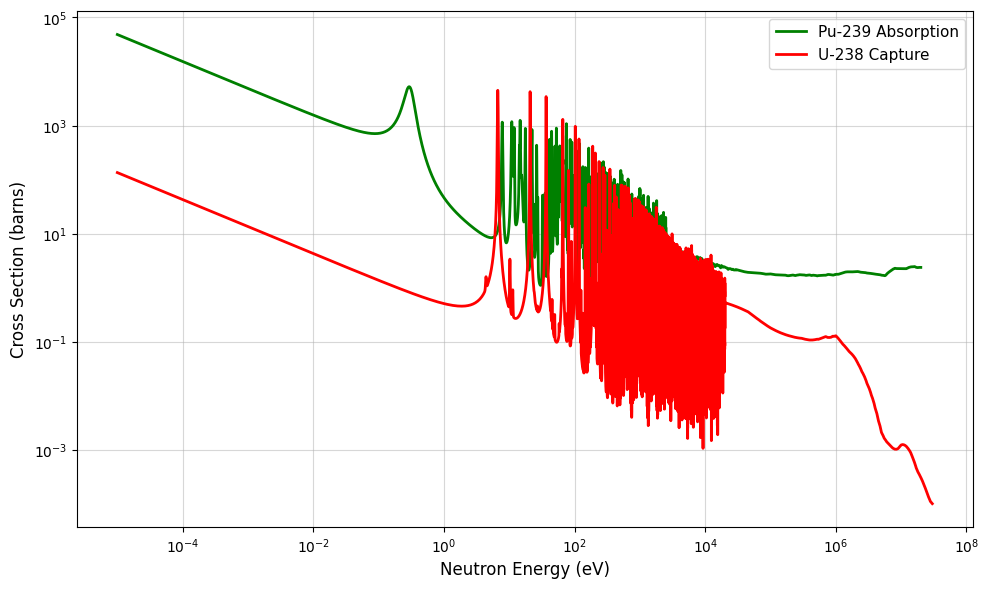
\includegraphics[width=0.75\linewidth]{figs/breed_burn_xs.png}
    \caption{Neutron cross sections for $^{238}$U radiative capture (breeding) and $^{239}$Pu absorption (burning) as functions of energy, evaluated from ENDF/B-VIII.0 at 900\,K \cite{Brown2018ENDF/B-VIII.0:Data}. In the thermal range, $\sigma_\text{a,Pu239}$ exceeds $\sigma_{(n,\gamma),\text{U238}}$ by two to three orders of magnitude, establishing the physical basis for the LBR's thermal spectrum strategy.}
    \label{fig:breed-burn-xs}
\end{figure}

% ============================================================
\subsection{Preliminary Neutronics Scoping}
\label{sec:scoping}
% ============================================================

The cross-section analysis establishes the need for a highly thermalized spectrum but does not by itself determine the moderator material or lattice geometry. A series of preliminary scoping calculations was performed --- progressing from infinite lattice models to 0-D depletion analyses --- to translate the spectrum requirement into concrete design parameters.

\subsubsection{Moderator and Lattice Pitch: Infinite Lattice Study}

An infinite lattice model was constructed using a representative high-burnup TMI-1 spent fuel composition (52.6\,GWd/tHM --- one of the highest-burnup samples available in the SFCOMPO-2.0 database \cite{Michel-Sendis2017SFCOMPO-2.0:Data}), chosen as a conservative baseline that maximizes the challenge of sustaining criticality with degraded fuel. Three moderator candidates were evaluated --- light water (H$_2$O), heavy water (D$_2$O), and helium --- across a range of lattice pitches from 1.5 to 15\,cm.

\begin{figure}[H]
    \centering
    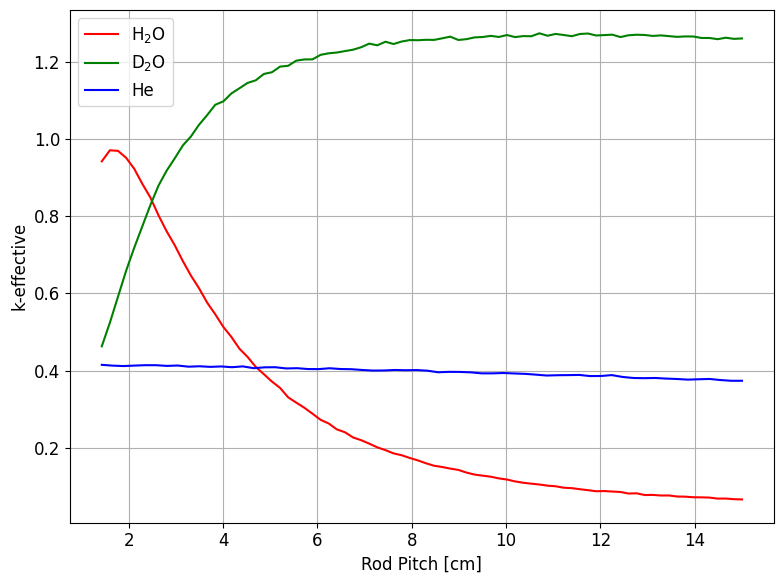
\includegraphics[width=0.73\linewidth]{figs/KinfVsPitch.png}
    \caption{Infinite multiplication factor $k_\infty$ at startup versus lattice pitch for H$_2$O, D$_2$O, and He moderation, using a representative TMI-1 spent fuel composition (52.6\,GWd/tHM). Light water and helium fail to achieve criticality at any pitch; D$_2$O reaches $k_\infty > 1$ for pitches above $\sim$3\,cm and plateaus near 1.27 at 6--15\,cm.}
    \label{fig:kinf-pitch}
\end{figure}

\begin{figure}[H]
    \centering
    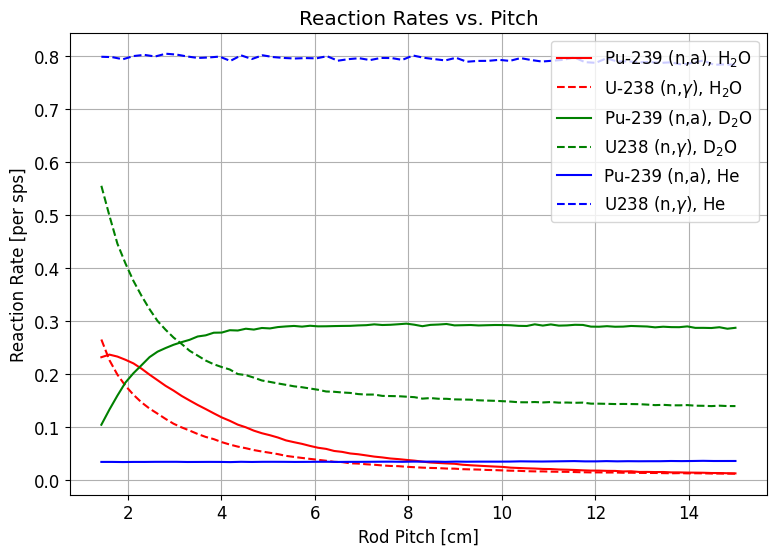
\includegraphics[width=0.73\linewidth]{figs/RRvsPitch.png}
    \caption{Normalized $^{239}$Pu absorption (burning) and $^{238}$U capture (breeding) reaction rates versus lattice pitch for H$_2$O and D$_2$O moderation. Heavy water uniquely sustains a configuration where the burning rate exceeds the breeding rate ($\lambda_3 > \lambda_2$) over a broad pitch range, confirming D$_2$O as the only viable moderator for net plutonium reduction.}
    \label{fig:breed-burn-rr}
\end{figure}

As shown in Figure~\ref{fig:kinf-pitch}, light water and helium moderation fail to sustain criticality at any pitch using spent fuel of this burnup. Heavy water is the only candidate that achieves $k_\infty > 1$, owing to its low thermal neutron absorption cross section ($\sigma_\text{a,D2O} \approx 0.001$\,b) compared to light water ($\sigma_\text{a,H2O} \approx 0.33$\,b), which preserves neutron economy in a fuel-poor lattice. The reaction rate comparison in Figure~\ref{fig:breed-burn-rr} confirms that only the D$_2$O system achieves the burning-over-breeding condition across a broad pitch range.

A lattice pitch of 6\,cm was selected as the baseline design point, providing a balance between three competing requirements:
\begin{enumerate}
    \item Sufficient spectrum thermalization to maintain $\lambda_3/\lambda_2 > 1$ (Objective~1: plutonium burning).
    \item Adequate initial excess reactivity ($k_\infty \approx 1.22$) to sustain criticality throughout the fuel cycle (Objective~2).
    \item Acceptable moderator-to-fuel ratio from a thermal-hydraulic standpoint (Objective~3), discussed further in Section~\ref{sec:thermalhydraulics}.
\end{enumerate}

\subsubsection{Zero-Dimensional Depletion Analysis}

Having established the D$_2$O / 6\,cm pitch design point, a zero-dimensional (0-D) depletion analysis was performed to assess cycle length, plutonium burndown, and isotopic quality degradation under continuous irradiation at constant power. A power density of 30\,W/gHM was selected, consistent with typical PWR operation and yielding a total heavy metal inventory of approximately 67\,tonnes at 2\,GW$_\text{th}$ across $\sim$19\,400 fuel rods.

\paragraph{Burnup Constraint.}
The NRC regulatory burnup limit is 62\,GWd/tHM. Starting from an initial burnup of 52.6\,GWd/tHM leaves a margin of 9.4\,GWd/tHM, corresponding to a maximum operation time of:
\begin{equation}
    T_\text{max} = \frac{9.4\ \text{GWd/tHM}}{30\ \text{W/gHM}} = 313\ \text{days}
\end{equation}

\begin{figure}[H]
    \centering
    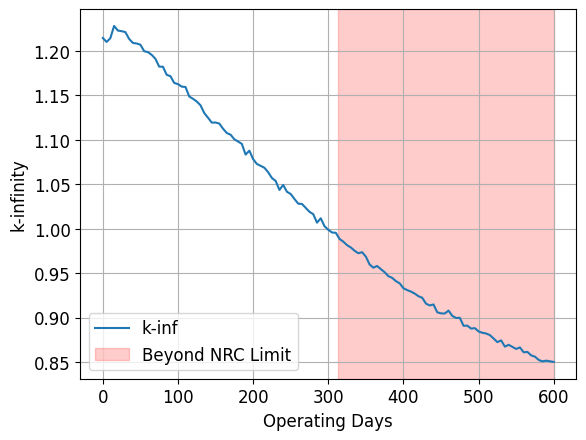
\includegraphics[width=0.8\linewidth]{figs/kinfVsBurn.png}
    \caption{Infinite multiplication factor $k_\infty$ versus operating time at 30\,W/gHM for the D$_2$O / 6\,cm pitch infinite lattice. Criticality is maintained for 300 days --- 13 days short of the NRC burnup limit --- demonstrating near-optimal utilization of available reactivity margin. The shaded region indicates operation beyond the regulatory burnup ceiling.}
    \label{fig:kinf-burn}
\end{figure}

Figure~\ref{fig:kinf-burn} shows that $k_\infty \geq 1$ is maintained for 300 days, 13 days (4\%) short of the burnup-limited maximum. This indicates near-optimal fissile utilization within regulatory constraints. The initial excess reactivity ($k_\infty = 1.22$) would be managed through soluble boron, control rods, or burnable poisons in the finite reactor.

\paragraph{Fissile Inventory Evolution.}

\begin{figure}[H]
    \centering
    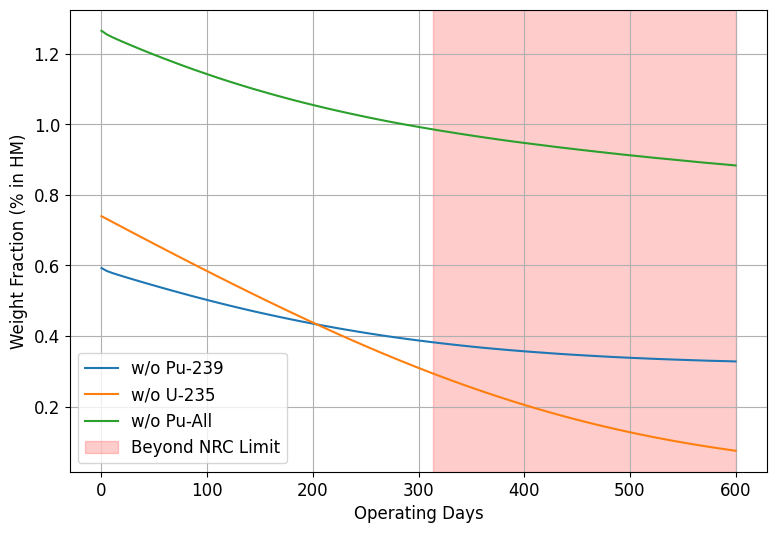
\includegraphics[width=0.8\linewidth]{figs/concVsBurn.png}
    \caption{Fissile isotope weight fractions versus operating time. $^{235}$U depletes from 0.74\% to 0.30\% (59\% reduction) while $^{239}$Pu depletes from 0.59\% to 0.39\% (34\% reduction). Total plutonium decreases from 1.26\% to 0.99\% --- a 21.5\% reduction, exceeding the 20\% design target. Continuous breeding from $^{238}$U partially replenishes the $^{239}$Pu inventory, consistent with the $\lambda_3/\lambda_2 > 1$ condition.}
    \label{fig:conc-burn}
\end{figure}

Figure~\ref{fig:conc-burn} confirms net plutonium burning: total plutonium decreases by 21.5\% over the operating cycle, destroying approximately 16\,kg of plutonium per tonne processed, or $\sim$1\,070\,kg total for the full core.

\paragraph{Plutonium Isotopic Quality Degradation.}

\begin{figure}[H]
    \centering
    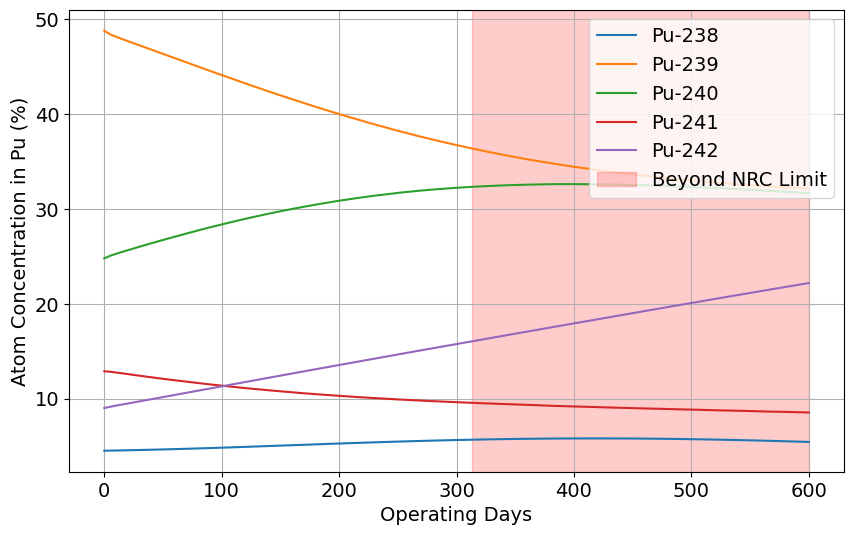
\includegraphics[width=0.8\linewidth]{figs/attractiveness.png}
    \caption{Plutonium isotopic composition versus operating time. The fissile isotopes $^{239}$Pu and $^{241}$Pu decrease while $^{238}$Pu, $^{240}$Pu, and $^{242}$Pu increase, progressively degrading the material's weapons attractiveness through elevated decay heat, higher spontaneous fission rates, and reduced fissile fraction.}
    \label{fig:attractiveness}
\end{figure}

Figure~\ref{fig:attractiveness} shows the evolution of individual plutonium isotopes. The relative $^{239}$Pu fraction decreases by 24.7\%, while $^{240}$Pu (high spontaneous fission rate) increases by 30.0\% relative to total plutonium. This isotopic shift simultaneously reduces net fissile content and increases self-heating and neutron emission rates, all of which degrade the material's utility for weapons applications even if chemically separated.

\paragraph{0-D Scoping Summary.}
The 0-D infinite lattice analysis confirms that all three primary design objectives are achievable at the scoping level:
\begin{itemize}
    \item \textbf{Plutonium reduction}: 21.5\% total Pu mass decrease, exceeding the $\geq$20\% target.
    \item \textbf{Cycle length}: 300 days at full power, exceeding the $\geq$270-day target.
    \item \textbf{Isotopic degradation}: $^{240}$Pu fraction increased 30\%, substantially reducing weapons attractiveness.
\end{itemize}

These results assume spatially uniform depletion and an ideal infinite lattice. Several critical phenomena are outside the scope of 0-D analysis and require higher-fidelity treatment before the design can be considered credible:

\begin{enumerate}
    \item \textbf{Axially non-uniform spent fuel burnup.} Real PWR assemblies discharge with a spatially varying burnup profile --- the rod extremities retain substantially more fissile material than the axial midplane. A 0-D model cannot capture this, so the isotopic starting conditions for the LBR differ significantly from those of a single-composition infinite lattice.
    \item \textbf{Isotopic validation.} The 0-D model uses a single tabulated composition from a database. Before those compositions can be trusted as LBR fuel inputs, the depletion code must be benchmarked against measured post-irradiation examination (PIE) data.
    \item \textbf{Spectral coupling between moderator and fuel.} The interaction between the D$_2$O moderator and spatially distributed fuel regions in a real assembly changes both the effective pitch and the flux-weighted cross sections relative to the infinite lattice assumption.
    \item \textbf{Axial power redistribution.} The non-uniform fissile profile drives an axially peaked power distribution that is invisible to 0-D models but directly impacts cycle length, thermal margins, and fuel utilization efficiency.
\end{enumerate}

These limitations establish the scope of the detailed Monte Carlo analyses presented in Section~\ref{sec:neutronics}: (i)~a Serpent~2 depletion model of Assembly NJ05YU from TMI-1 is benchmarked against measured isotopic data to validate the spent fuel compositions; (ii)~a full assembly Serpent lattice model replaces the infinite lattice approximation for moderator and pitch selection; and (iii)~an iterative design study identifies and optimizes a power-redistribution strategy to address the axial burnup non-uniformity that the scoping analysis could not resolve.
